\documentclass[conference]{IEEEtran}
\IEEEoverridecommandlockouts

\usepackage{cite}
\usepackage{amsmath,amssymb}
\usepackage{graphicx}
\usepackage{booktabs}
\usepackage{multirow}
\usepackage{xcolor}
\usepackage{url}
\usepackage{tikz}
\usetikzlibrary{arrows.meta,positioning,fit,calc}

\definecolor{actblue}{HTML}{2A78D6}
\definecolor{ikorange}{HTML}{EB6834}
\definecolor{vlaaqua}{HTML}{1BAF7A}
\definecolor{muted}{HTML}{52514E}

\usepackage{xspace}
\usepackage{algorithm}
\usepackage{algorithmic}
\newcommand{\mm}{\,mm\xspace}

\begin{document}

\title{WildTrace: Photo-to-Pen Robot Drawing with Learned Path-Following Policies and a Calibrated Digital Twin}

\author{
\IEEEauthorblockN{Author One, Author Two, Author Three}
\IEEEauthorblockA{Affiliation\\
City, Country\\
\{author\}@example.edu}
}

\maketitle

\begin{abstract}
We present WildTrace, an end-to-end system that turns photographs of animals and faces into pen-stroke
trajectories and draws them with a 7-DoF UFACTORY xArm~7, both in a calibrated NVIDIA Isaac Sim twin and on the
physical arm. A medallion data pipeline uses a diffusion model to redraw each photo as a clean outline, a
vision-language judge with OpenCV prescreening to reject bad outlines, and a vectoriser that emits a few
ordered strokes, yielding 2,874 validated trajectories over six animal classes. On top of this data we train an
Action Chunking Transformer (ACT) that maps joint state and a short window of the upcoming path to joint steps,
using only kinematic inverse-kinematics labels with noise injection. On a held-out set of 48 drawings in the
twin at 1\,g, ACT finishes 48/48 drawings against 45/48 for a Lula IK baseline, lowers mean path RMSE from
0.277\mm to 0.192\mm (lower on all 45 paired drawings, Wilcoxon $p<10^{-12}$), halves joint jerk, and is
unaffected by $\pm$12\mm paper height and 21\mm planar placement errors. A streaming IK baseline without the
settle gate gains only 0.010\mm, so the improvement comes from the learned policy. A fine-tuned SmolVLA
re-planned every tick is slightly more accurate still (0.180\mm) but jerkier and twice as slow to query, and a
rule-based supervisor that hands stalls and ink gaps to IK repairs
injected ink skips (87 redraws for 105 skips, none abandoned) at under 0.011\mm cost. On the physical arm, ACT completes 30/30 animal drawings at
0.532\mm RMSE and three face portraits at 0.497\mm, about 2.7$\times$ the twin, a gap that we analyse.
\end{abstract}

\begin{IEEEkeywords}
robot drawing, imitation learning, action chunking, vision-language-action models, digital twin, sim-to-real
\end{IEEEkeywords}

%======================================================================
\section{Introduction}
%======================================================================

Robot drawing is a compact testbed for precise contact-rich path following: the pen must stay on a sheet a
fraction of a millimetre away, follow tight curves without overshoot, and lift and land cleanly between
strokes. Every error is visible on paper. Classic pipelines solve inverse kinematics (IK) per waypoint and
wait for the arm to settle~\cite{calinon2005humanoid,tresset2013paul}, which is reliable but slow and leaves a
visible tremor. Learned visuomotor policies such as ACT~\cite{zhao2023act}, diffusion
policy~\cite{chi2023diffusion} and vision-language-action (VLA) models such as SmolVLA~\cite{shukor2025smolvla}
promise smoother motion, but are usually evaluated by task success rather than by sub-millimetre path accuracy
on open-ended content.

WildTrace closes the loop from an arbitrary photograph to ink on paper (Fig.~\ref{fig:pipeline}) and uses it to
compare controllers on the same drawings under identical physics. Our contributions are:
\begin{enumerate}
  \item A photo-to-trajectory pipeline with a generate-judge-retry loop, which we use to build 2,874 validated
        drawing trajectories and a 48-drawing held-out test set (Sec.~\ref{sec:pipeline}).
  \item A path-conditioned ACT policy trained only on kinematic IK labels with noise injection and a capped
        progress projection, which beats IK in a calibrated 1\,g twin on accuracy, completion and smoothness,
        is insensitive to paper placement, and keeps its lead over a streaming IK baseline that shares its
        progress rule and pace (Sec.~\ref{sec:control},~\ref{sec:results}).
  \item A like-for-like comparison with a fine-tuned SmolVLA on the same data: re-planned every tick it matches
        and slightly exceeds ACT on the test set, at higher jerk and latency, and a negative result on
        camera-conditioned gap repair.
  \item A hybrid supervisor that repairs skipped ink using the run's own bookkeeping, and a physical-arm
        evaluation on 30 animal drawings and three portraits that quantifies the sim-to-real gap.
\end{enumerate}

\begin{figure*}[t]
  \centering
  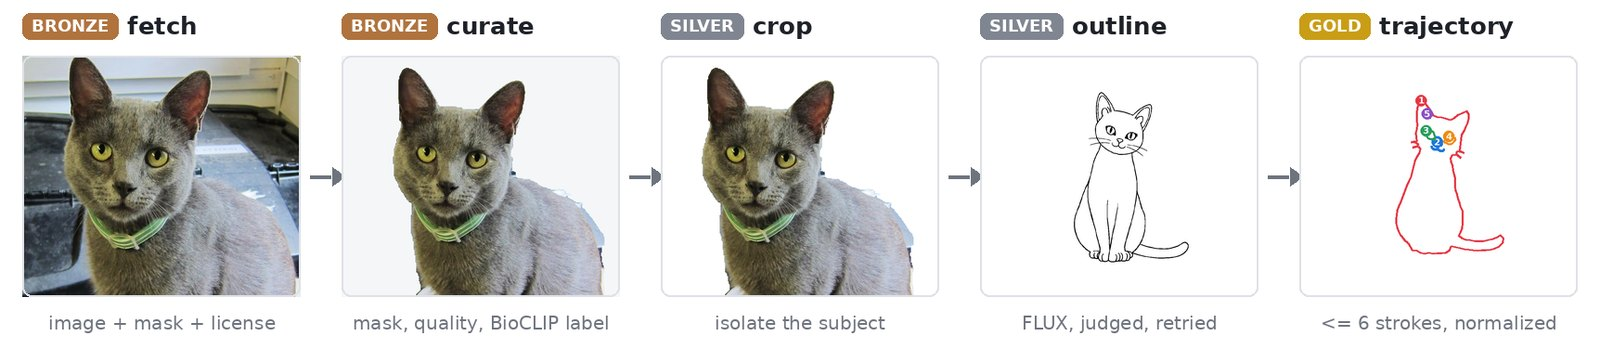
\includegraphics[width=\textwidth]{figures/pipeline.jpg}
  \caption{WildTrace data pipeline on one Open Images~\cite{kuznetsova2020openimages} photo. Bronze: fetch the
  image, mask and license, then curate and label (BioCLIP~\cite{stevens2024bioclip}). Silver: isolate the subject
  and redraw it as an outline with FLUX~\cite{flux2024}, judged and retried. Gold: the accepted outline becomes a
  few ordered pen strokes on a normalised canvas (numbered markers show stroke starts).}
  \label{fig:pipeline}
\end{figure*}

%======================================================================
\section{Related Work}
%======================================================================

\textbf{Robot drawing and painting.} Portrait-drawing robots date back to humanoid systems that extract contours
and replay them with IK~\cite{calinon2005humanoid} and to Paul, which emulates an artist's sketching
process~\cite{tresset2013paul}. Recent systems differ mainly in what they draw and how fast. RoboCoDraw turns a
face into a GAN avatar and orders its strokes with a genetic algorithm, drawing in 43\,s on a
UR5~\cite{wang2019robocodraw}; AiSketcher draws synthesised portraits with a 3-DoF arm in about two
minutes~\cite{gao2020aisketcher}; Nasrat et al.\ draw portraits in 80\,s with line width set by pen
height~\cite{nasrat2023artistic}; Piktor-O-Bot adds force-controlled shading on a UR5 and shapes speed by path
curvature~\cite{hoang2024piktor,csempesz2024piktor}; TSP-Bot draws single-path stipple art with
TRAC-IK~\cite{song2022tspbot}; and line art can be parsed into stroke graphs for a desktop
arm~\cite{venkataramaiyer2020lineart}. These systems execute planned paths and report drawing time, style or
viewer preference rather than tracking accuracy. Learned stroke models~\cite{ha2018sketchrnn,huang2019paint}
plan in image space, and FRIDA~\cite{schaldenbrand2023frida} and Spline-FRIDA~\cite{chen2024splinefrida}
learn stroke appearance to shrink the sim-to-real gap of the painted image. Closest to our control question,
Lee et al.\ learn motor control with hierarchical reinforcement learning instead of IK, but need pen-tip
feedback to correct the learned controller on a real UR5e~\cite{lee2022scratch}. We take the strokes as given
and measure how precisely learned policies follow them against IK, at sub-millimetre resolution.

\textbf{Imitation learning for fine control.} ACT~\cite{zhao2023act} predicts chunks of future actions with a
transformer; diffusion policy~\cite{chi2023diffusion} models multimodal action distributions. DART~\cite{laskey2017dart}
injects noise during demonstration to cover off-path states and DAgger~\cite{ross2011dagger} aggregates on-policy
corrections. We use DART-style noise with a synthetic IK teacher, and DAgger rounds for camera policies.

\textbf{Vision-language-action models.} SmolVLA~\cite{shukor2025smolvla} reuses a pretrained vision-language
backbone for control, with a flow-matching action head~\cite{lipman2023flow}. We fine-tune SmolVLA on the same data as ACT to test whether a pretrained
generalist helps a precision task.

\textbf{Sim-to-real.} Domain randomisation~\cite{tobin2017domain} widens the training distribution to cover the
real system; we instead calibrate the twin to the lab arm and randomise only paper placement.

%======================================================================
\section{Data Pipeline: Photo to Pen Strokes}
\label{sec:pipeline}
%======================================================================

The pipeline is a local-first medallion design with one script per stage and append-only NDJSON manifests,
so a stage reruns only for rows whose configuration or input hash changed.

\textbf{Bronze.} Images, segmentation masks and licenses are fetched from Open Images V7 for six classes (bird,
cat, dog, fish, frog, horse), de-duplicated, filtered for quality and viewing angle, and labelled with BioCLIP.

\textbf{Silver.} The subject is cropped by its mask and redrawn as a black-on-white outline by FLUX.1-schnell.
A LangGraph~\cite{langgraph} loop validates each outline with an OpenCV prescreen (foreground ratio, component
count, contour size, fragmentation) followed by a VLM judge, and retries with a new seed on failure.

\textbf{Gold.} The best outline per pose is skeletonised and vectorised into a few ordered strokes,
resampled and normalised to a unit canvas. The result is 2,874 validated trajectories. A stratified 48-drawing
gold test set (9 bird, 12 cat, 13 dog, 4 fish, 5 frog, 5 horse; mean 4.6 strokes, range 2 to 8, mean 370
points) is never used for training. Faces follow a separate CPU path: MediaPipe~\cite{lugaresi2019mediapipe} face
landmarks and hair/body segmentation are traced into a pen-sketch portrait. Fig.~\ref{fig:faces} shows five portraits from this path
next to their source photographs.

\begin{figure*}[t]
  \centering
  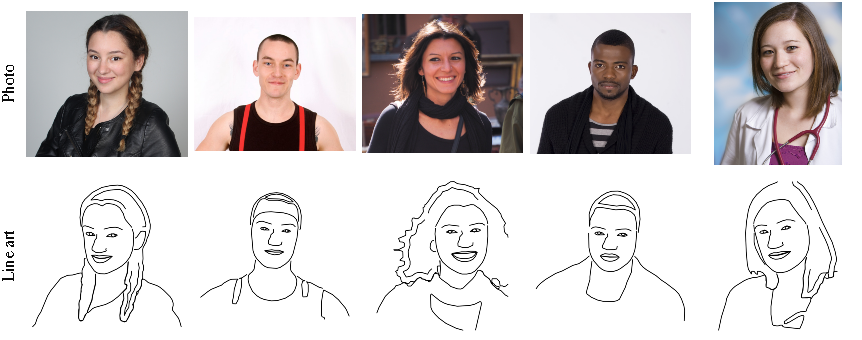
\includegraphics[width=\textwidth]{figures/faces.pdf}
  \caption{Face portraits: Open Images source photographs (top) and the pen-sketch line art traced from MediaPipe
  landmarks and segmentation (bottom), 15 to 19 strokes each. Photographs CC BY 2.0 via Flickr, by Byron Gonzalez,
  MangakaMaiden Photography, Luca Boldrini, JJP Bolger Photography and Walt Stoneburner (left to right).}
  \label{fig:faces}
\end{figure*}

\textbf{Choosing the generator and the judge.} Table~\ref{tab:judge} summarises a 20-subject study against a
strong referee (Qwen3-VL-235B~\cite{bai2025qwen3vl}). FLUX produced acceptable outlines for all 20 subjects against
6/20 for OmniGen2~\cite{wu2025omnigen2} (paired sign test $p=10^{-4}$), whose failures were mostly blank pages. The local Qwen2.5-VL-7B~\cite{bai2025qwen25vl} judge originally
in production agreed with the referee no better than chance and passed every blank page; we therefore switched
to Qwen3-VL-8B, which agrees with the referee on 92.5\% of outlines.

\textbf{Why open-weight models, not frontier APIs.} Every generator and judge in the pipeline is an open-weight
model that runs on the lab's single 16\,GB laptop GPU, and we did not evaluate proprietary frontier models in
either role. Four reasons drove this. (i) \emph{Volume and cost}: the dataset took thousands of generate-judge
calls with up to three attempts per subject, at zero marginal cost locally; a hosted open 8B judge costs about
\$0.00004 per call, which keeps even hosted runs negligible. (ii) \emph{Privacy}: WildTrace Studio turns
uploaded photographs of people into portraits, and a local pipeline never sends those faces to a third party.
(iii) \emph{Reproducibility}: pinned open weights give the same verdicts on a rerun, whereas a hosted frontier
model can change under the same name. (iv) \emph{Sufficiency}: an 8B open judge already agrees with a 235B open
referee at $\kappa=0.83$, so a larger judge has little room to improve the accept/reject decision. The cost is
that we cannot report how a frontier judge would score; the referee is itself an open model.

\begin{table}[t]
\centering
\caption{Outline generator and judge study (20 subjects, referee Qwen3-VL-235B).}
\label{tab:judge}
\setlength{\tabcolsep}{4pt}
\begin{tabular}{lcc}
\toprule
Generator & Referee pass & BioCLIP top-1 \\
\midrule
FLUX.1-schnell & \textbf{20/20} & \textbf{75\%} \\
OmniGen2       & 6/20  & 30\% \\
\midrule
Judge & Agreement & Cohen's $\kappa$ \\
\midrule
Qwen2.5-VL-7B (local) & passes 9/9 blanks & 0.00 \\
Qwen3-VL-8B           & \textbf{92.5\%}   & \textbf{0.83} \\
\bottomrule
\end{tabular}
\end{table}

%======================================================================
\section{Robot, Twin and Controllers}
\label{sec:control}
%======================================================================

\begin{figure}[t]
  \centering
  \setlength{\tabcolsep}{1pt}
  \begin{tabular}{ccc}
    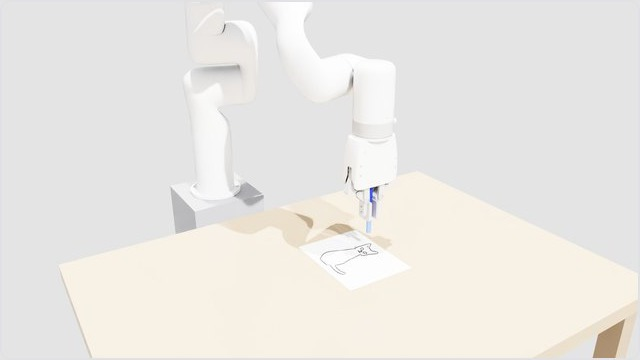
\includegraphics[height=2.38cm]{figures/twin_scene.jpg} &
    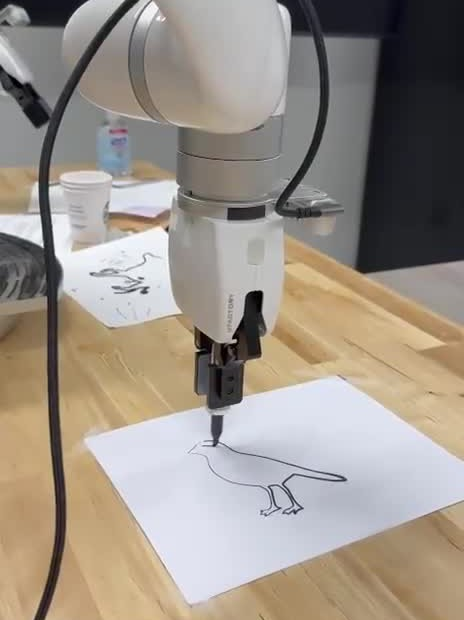
\includegraphics[height=2.38cm]{figures/real_arm.jpg} &
    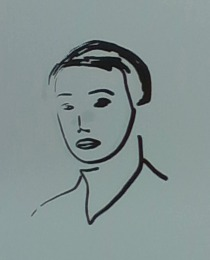
\includegraphics[height=2.38cm]{figures/real_face.jpg} \\
    \footnotesize (a) Lab-arm twin & \footnotesize (b) Physical xArm 7 & \footnotesize (c) Real portrait
  \end{tabular}
  \caption{(a) Isaac Sim twin built from the lab arm's calibrated URDF, gripper and measured paper placement, at
  1\,g. (b) The physical xArm 7 drawing a WildTrace bird. (c) A face portrait drawn by ACT on the physical arm
  with a marker (run 7 in Table~\ref{tab:real}).}
  \label{fig:robot}
\end{figure}

\textbf{Hardware and twin.} A UFACTORY xArm 7 holds a pen in its parallel gripper over a US Letter sheet. The
Isaac Sim~\cite{isaacsim} twin (Fig.~\ref{fig:robot}a) uses the arm's calibrated URDF, the measured paper pose and pen touch height,
Earth gravity, and a stiff PhysX position servo (stiffness $7.5\times10^5$, damping 2050) standing in for the
vendor joint controller. Two RealSense D435i cameras (wrist and overhead) were located by depth plane fitting
and planar PnP on the sheet corners, whose heights above the paper agree to within 1.6\%. Each drawing runs a fixed phase machine:
approach, lower, draw, lift for every stroke, with short pen-up hops between nearby strokes.

\textbf{Metrics.} Let $\{p_i\}_{i=1}^{N}$ be the planned pen-down samples and $\{e_j\}$ the executed
pen-down pen-tip positions, both in 3-D. The nearest-path error of a planned sample is
\begin{equation}
  d_i = \min_j \lVert p_i - e_j \rVert_2 ,
  \label{eq:dist}
\end{equation}
and we report the path RMSE $\big(\tfrac{1}{N}\sum_i d_i^2\big)^{1/2}$, the 95th percentile and the maximum of
$d_i$. Because (\ref{eq:dist}) only penalises missing a planned point, we also report the reverse direction,
from each executed sample to the plan, which catches stray ink. Joint jerk is the RMS over pen-down samples of
$\lVert \Delta^3 q \rVert / \Delta t^3$, the third difference of joint positions within a stroke. Corner RMSE
is the tracking error at waypoints flagged as corners, and heading error compares the direction of plan and pen
over a 4\mm chord.

\textbf{IK baseline.} NVIDIA Lula IK solves joint targets for each waypoint of the resampled path (at most
5\mm apart, densified at corners); joint commands are slew-limited, and the run advances only when the measured
tip is within tolerance and its velocity has settled. A waypoint timeout fails the drawing safely. This is the
controller the system shipped with and the teacher that labels the policy data.

\textbf{Streaming IK baseline.} To separate learning from the settle gate, a second IK baseline uses exactly
ACT's progress rule (the first waypoint ahead of the pen's projection, Sec.~\ref{sec:control}) with no settle
gate, and solves Lula IK every tick for a carrot a fixed arc length $L$ ahead of the pen (pure pursuit). The carrot
advances along the path no faster than ACT's median pen speed, 12.4\mm\,s$^{-1}$, so both controllers draw at
the same pace; we also run it at plain IK's median pen speed, 6.9\mm\,s$^{-1}$. On six drawings outside the test
set, $L$ between 0.5 and 2\mm made no difference because the speed limit binds, so we use $L=0.5$\mm. Without
the speed limit, pure pursuit raced through a drawing in a sixth of the time at 0.69\mm RMSE.

\textbf{ACT path follower.} At control tick $t$ the policy observes the robot state
$s_t = [\,q_t,\ \dot q_t,\ u_{t-1}\,] \in \mathbb{R}^{21}$ (joint positions, velocities and previous joint
command) and a path context
\begin{equation}
  c_t = \big[\,x_t,\ g_t - x_t,\ \{w_{t,k} - x_t\}_{k=1}^{10},\ \pi_t\,\big] \in \mathbb{R}^{37},
\end{equation}
where $x_t$ is the pen tip, $g_t$ the current target, $w_{t,k}$ ten points spaced at equal arc length along the
next 2\,cm of path, and $\pi_t$ the pen state. It predicts a chunk of $H=10$ joint \emph{increments}
$\hat\delta_{t:t+H-1}$, trained with an L1 loss against the teacher's increments, and only the first is
executed:
\begin{equation}
  u_t = u_{t-1} + \alpha\, \hat\delta_t , \qquad \alpha = 0.5 .
  \label{eq:step}
\end{equation}
Absolute joint targets were mm-imprecise even when overfitting one drawing, so the policy predicts increments.
There is no image input. We use ACT~\cite{zhao2023act} via LeRobot~\cite{lerobot2024} with $d=256$, 4
encoder and 1 decoder layers, no CVAE, no dropout, learning rate $3\times10^{-4}$, batch 256 and 40k steps. On a
single-drawing overfit gate these choices cut first-action error from 33-45\% to 11\% of the label, a 10-step
chunk fit 2.5$\times$ better at p95 than a 30-step chunk, and executing only the first action of each chunk
with re-planning every tick tracked better than temporal ensembling. At run time the policy is queried at
60\,Hz and half of each predicted step is applied.

\textbf{Labels without physics.} Labels come from Lula IK walked through the same phase machine with no
physics simulation (about 20k solves/s), three episodes per training drawing. Two of the three add DART-style
command noise~\cite{laskey2017dart} and a measured-versus-commanded joint offset, so the policy sees sagged,
off-path states with the corrective label. Path progress is the projection of the tip onto the path, capped
at 1.5\mm ahead; without the cap progress jumped across narrow hairpins (8.1\mm worst-point error on one
frog toe) and spike tips were rounded. The lab-arm model is trained with $\pm$15\mm paper-height jitter.
Fine-tuning on 1\,g Isaac IK rollouts made tracking worse (0.74 to 0.91\mm on four drawings), because those
labels carry IK's own sag.

\textbf{SmolVLA.} We fine-tune SmolVLA~\cite{shukor2025smolvla} on the same dataset (19.8M frames), feeding the
full 58-value state through a direct-state MLP, 8 VLM layers, 256\,px rendered path images and 20-action chunks
(51M of 323M parameters trained). It is served with zero initial noise (better than averaging samples
offline); with 3 flow-matching steps, a captured CUDA graph cuts sampling from about 225\,ms to 30\,ms per
chunk.

\textbf{Hybrid supervisor.} A rule-based supervisor (Algorithm~\ref{alg:sup}, Fig.~\ref{fig:arch}) watches
the run's own ink bookkeeping rather than the policy. If the drawing target has not advanced for 1.5\,s, IK drives
the next 5\mm and hands back. If at least 1.5\mm of path behind the pen has no ink within 1\mm (the labeller's
coverage rule), IK goes back past the gap and forward again while the run's progress is held, then the policy
resumes. Both rules need no camera, so they also work on the physical arm.

\begin{algorithm}[t]
\caption{Hybrid supervisor, run every control tick}
\label{alg:sup}
\begin{algorithmic}[1]
\REQUIRE policy $\pi$, path progress $s$, inked set $\mathcal{I}$, last advance time $t_a$
\IF{$t - t_a > 1.5$\,s}
  \STATE drive the next 5\mm of path with Lula IK; $t_a \leftarrow t$ \COMMENT{stall}
\ELSIF{a stretch $[s_0, s_1] \subset [0, s]$ with $s_1 - s_0 \ge 1.5$\,mm has no ink within 1\mm}
  \STATE hold $s$; IK goes back to $s_0$, retraces to $s$ \COMMENT{gap}
  \STATE add the retraced path to $\mathcal{I}$; give up after a timeout
\ELSE
  \STATE $u_t \leftarrow u_{t-1} + \alpha\,\pi(s_t, c_t)_1$ \COMMENT{policy, Eq.~(\ref{eq:step})}
\ENDIF
\STATE update $s$ by projecting the tip onto the path (capped at 1.5\mm ahead)
\end{algorithmic}
\end{algorithm}

\begin{figure}[t]
\centering
\resizebox{\columnwidth}{!}{%
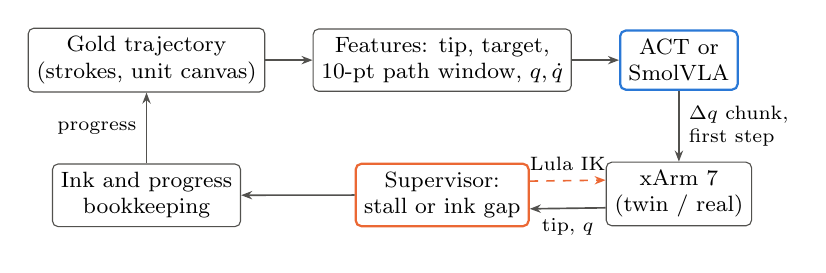
\begin{tikzpicture}[
  font=\footnotesize,
  box/.style={draw=muted, rounded corners=2pt, align=center, minimum height=0.75cm, inner sep=3pt, fill=white},
  arr/.style={-{Stealth[length=4pt]}, draw=muted, line width=0.6pt}]
  \node[box] (traj) {Gold trajectory\\(strokes, unit canvas)};
  \node[box, right=0.6cm of traj] (feat) {Features: tip, target,\\10-pt path window, $q,\dot q$};
  \node[box, right=0.6cm of feat, draw=actblue, line width=0.8pt] (pol) {ACT or\\SmolVLA};
  \node[box, below=0.9cm of pol] (sim) {xArm 7\\(twin / real)};
  \node[box, below=0.9cm of feat, draw=ikorange, line width=0.8pt] (sup) {Supervisor:\\stall or ink gap};
  \node[box, below=0.9cm of traj] (ink) {Ink and progress\\bookkeeping};
  \draw[arr] (traj) -- (feat);
  \draw[arr] (feat) -- (pol);
  \draw[arr] (pol) -- node[right, align=left, font=\scriptsize]{$\Delta q$ chunk,\\first step} (sim);
  \draw[arr] ([yshift=-5pt]sim.west) -- node[below, font=\scriptsize]{tip, $q$} ([yshift=-5pt]sup.east);
  \draw[arr, dashed, draw=ikorange] ([yshift=5pt]sup.east) -- node[above, font=\scriptsize]{Lula IK} ([yshift=5pt]sim.west);
  \draw[arr] (sup) -- (ink);
  \draw[arr] (ink) -- node[left, font=\scriptsize]{progress} (traj);
\end{tikzpicture}}
\caption{Control loop. The policy runs every 60\,Hz tick on a path window around the current progress; the
supervisor hands control to Lula IK only on a stall or an uninked gap (dashed), then hands back.}
\label{fig:arch}
\end{figure}

%======================================================================
\section{Results}
\label{sec:results}
%======================================================================

All simulated runs use the lab-arm twin at 1\,g. The main comparison (Table~\ref{tab:gold}, Fig.~\ref{fig:kde})
runs all four controllers on all 48 gold drawings with the same code, scene and batch runner; per-run metrics and
plots are kept with the code.

\begin{table}[t]
\centering
\caption{Gold test set, 48 held-out drawings, lab-arm twin at 1\,g, same code and runner for all four
controllers. Means over finished drawings; 95\% bootstrap intervals over drawings in brackets. S-IK is the
streaming IK baseline at ACT's pace.}
\label{tab:gold}
\setlength{\tabcolsep}{2.2pt}
\footnotesize
\begin{tabular}{lcccc}
\toprule
Metric & Lula IK & S-IK & ACT & SmolVLA \\
\midrule
Finished & 45/48 & \textbf{48/48} & \textbf{48/48} & \textbf{48/48} \\
Path RMSE (mm) & 0.277 & 0.267 & 0.192 & \textbf{0.180} \\
\ \ 95\% CI & .271-.283 & .262-.272 & .190-.194 & .176-.184 \\
Path p95 (mm) & 0.398 & 0.373 & 0.335 & \textbf{0.327} \\
Path max (mm) & 0.778 & 0.953 & \textbf{0.776} & 0.871 \\
Reverse RMSE (mm) & 0.397 & 0.401 & 0.374 & \textbf{0.356} \\
Corner RMSE (mm) & 0.366 & 0.608 & \textbf{0.325} & 0.330 \\
Heading, median ($^\circ$) & 0.51 & \textbf{0.41} & 1.36 & 1.10 \\
Jerk RMS (rad\,s$^{-3}$) & 757 & 745 & \textbf{390} & 521 \\
Samples settling (\%) & 51 & 48 & 18 & \textbf{17} \\
Median speed (mm\,s$^{-1}$) & 6.9 & 7.8 & 12.4 & \textbf{14.1} \\
Sim. draw time (s) & 76.8 & 101.0 & 73.4 & \textbf{71.3} \\
Latency p50 (ms) & - & - & \textbf{9.1} & 17.7 \\
\bottomrule
\end{tabular}
\end{table}

\begin{table}[t]
\centering
\caption{Gold test set per class: mean path RMSE in mm (finished / total where not all finished).}
\label{tab:class}
\setlength{\tabcolsep}{4pt}
\begin{tabular}{lccccc}
\toprule
Class & $n$ & Lula IK & S-IK & ACT & SmolVLA \\
\midrule
Bird  & 9  & 0.266 & 0.260 & 0.191 & \textbf{0.184} \\
Cat   & 12 & 0.275 & 0.267 & 0.195 & \textbf{0.188} \\
Dog   & 13 & 0.282 (12) & 0.270 & 0.189 & \textbf{0.176} \\
Fish  & 4  & 0.295 (3) & 0.269 & 0.198 & \textbf{0.161} \\
Frog  & 5  & 0.289 (4) & 0.271 & 0.183 & \textbf{0.169} \\
Horse & 5  & 0.270 & 0.266 & 0.198 & \textbf{0.188} \\
\bottomrule
\end{tabular}
\end{table}

\begin{table}[t]
\centering
\caption{How the ACT path follower got there (48 gold drawings, 1\,g, means over finished drawings, runs made
during development with earlier code). Rows above the rule use the default sim scene, rows below the stiffened
lab-arm twin.}
\label{tab:ablation}
\setlength{\tabcolsep}{3pt}
\begin{tabular}{lcccc}
\toprule
Controller & Fin. & RMSE & Max & Jerk \\
\midrule
Lula IK & 39/48 & 0.698 & 0.985 & 806 \\
ACT, 30\,Hz, full step held 2 ticks & 48/48 & 0.366 & 2.599 & 1018 \\
\ \ + 60\,Hz queries, half step (Eq.~\ref{eq:step}) & 48/48 & 0.325 & 2.360 & 272 \\
\ \ + progress capped at 5\mm (hairpins) & 48/48 & \textbf{0.239} & 1.472 & \textbf{255} \\
\ \ + cap at 1.5\mm (spike tips) & 48/48 & 0.256 & \textbf{0.885} & 285 \\
\midrule
Lula IK, lab-arm twin & 44/48 & 0.283 & \textbf{0.775} & 752 \\
ACT, lab-arm twin, height jitter & \textbf{48/48} & \textbf{0.195} & 0.812 & \textbf{390} \\
\bottomrule
\end{tabular}
\end{table}

\begin{figure*}[t]
  \centering
  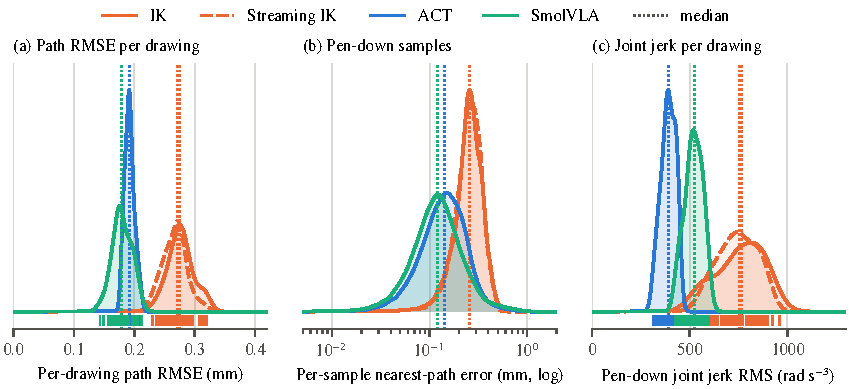
\includegraphics[width=\textwidth]{figures/kde_gold.pdf}
  \caption{Kernel density estimates (Gaussian kernel, Scott bandwidth) over the gold set for the four
  controllers; dotted lines are medians and ticks are individual drawings ($n$ = 45 / 48 / 48 / 48 drawings,
  71k / 76k / 76k / 76k pen-down samples for IK / streaming IK / ACT / SmolVLA). (a) Per-drawing path RMSE: the two
  learned policies separate cleanly from both IK variants. (b) Nearest-path error of every planned pen-down sample
  (densified plan): medians 0.256, 0.257, 0.141 and 0.120\mm. (c) Pen-down joint jerk: ACT is smoothest, SmolVLA
  between ACT and IK.}
  \label{fig:kde}
\end{figure*}

\begin{figure*}[t]
  \centering
  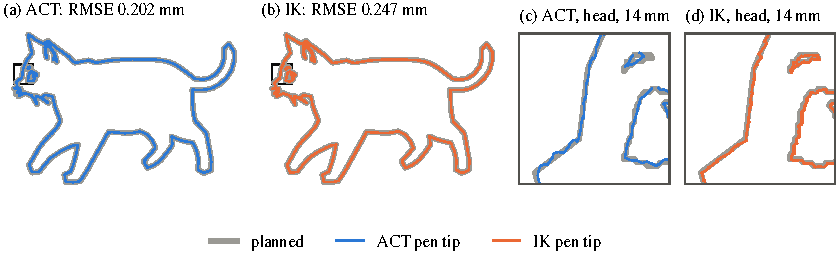
\includegraphics[width=\textwidth]{figures/paths_cat.pdf}
  \caption{Planned path (grey) against the executed pen tip for the same gold cat, ACT (blue) and IK (orange),
  top-down. (c, d) A fixed 14\mm window on the head: IK's stop-and-settle at each waypoint leaves a tremor of
  small hooks along the stroke; ACT stays smooth.}
  \label{fig:paths}
\end{figure*}

\textbf{ACT against IK.} ACT finishes every drawing; IK fails three on waypoint timeouts. On the 45 drawings both
finish, ACT has lower path RMSE on all 45: the paired reduction is 0.085\mm (95\% CI 0.079 to 0.091), or 31\%,
with two-sided Wilcoxon signed-rank $p=5.7\times10^{-14}$. The advantage holds in every class
(Table~\ref{tab:class}). It is not bought with stray ink: the reverse, pen-to-plan error is also lower (0.374
against 0.397\mm). Over pooled samples (Fig.~\ref{fig:kde}b) the median error falls from 0.256 to 0.141\mm.
ACT halves joint jerk (Fig.~\ref{fig:kde}c) and removes the per-waypoint tremor visible in Fig.~\ref{fig:paths}.
IK keeps a lower heading error (median 0.51$^\circ$ against 1.36$^\circ$), since it settles on each waypoint: its
pen is settling on 51\% of pen-down samples against 18\% for ACT, and moves at a median 6.9 against
12.4\mm\,s$^{-1}$. Total draw time is similar (77 against 73\,s simulated) because the phase machine's approach,
lower and lift moves are shared. The policy server answers in 9.1\,ms median, inside the 16.7\,ms tick. Retraining ACT with two more seeds gives 0.201 and 0.218\mm on the same 48 drawings
(three seeds: $0.204\pm0.013$\mm), all well below both IK variants.

\textbf{Is it the learning or the settle gate?} Streaming IK uses ACT's progress rule with no settle gate. It
finishes all 48 drawings (IK's timeouts came from the gate), but its path RMSE improves on IK by only 0.010\mm
(0.267\mm, lower on 37 of 45), its corner error grows from 0.366 to 0.608\mm because pure pursuit cuts corners,
and its jerk stays at IK's level. ACT is lower than streaming IK on all 48 drawings (paired reduction 0.075\mm,
CI 0.069 to 0.080). Slowing streaming IK to IK's own pace (carrot limit 6.9\mm\,s$^{-1}$) does not help:
0.266\mm RMSE, jerk down to 524 but corner error up to 0.973\mm, and 181\,s per drawing, still above ACT on all
48 drawings. Removing the gate is not what makes ACT accurate; the learned policy is.

\textbf{What mattered.} Table~\ref{tab:ablation} traces the design. Querying at 60\,Hz with half steps cut jerk
3.7$\times$; capping the progress projection fixed hairpin jumps (mean worst point 2.36 to 1.47\mm), and a tighter
cap fixed spike tips (0.885\mm) at a small RMSE cost. Moving to the stiffened lab-arm twin, with paper-height
jitter in training, gives the final policy. Each variant beats IK on path RMSE in its own scene.

\textbf{Paper placement.} Table~\ref{tab:robust} moves the sheet on a 16-drawing subset. ACT, trained with height
jitter, finishes all 64 runs within 0.189 to 0.193\mm. IK drops to 13/16 with the paper 12\mm lower and
degrades to 0.300\mm under a planar shift.

\begin{table}[t]
\centering
\caption{Paper placement robustness, 16 gold drawings (finished, mean path RMSE in mm).}
\label{tab:robust}
\setlength{\tabcolsep}{4pt}
\begin{tabular}{lcccc}
\toprule
Placement & \multicolumn{2}{c}{Lula IK} & \multicolumn{2}{c}{ACT} \\
\midrule
Nominal                & 15/16 & 0.278 & 16/16 & 0.192 \\
12\mm lower            & 13/16 & 0.284 & 16/16 & 0.189 \\
12\mm higher           & 15/16 & 0.271 & 16/16 & 0.193 \\
Shifted $(+15,-15)$\mm & 16/16 & 0.300 & 16/16 & 0.190 \\
\bottomrule
\end{tabular}
\end{table}

\textbf{SmolVLA against ACT.} On the full gold set with the batch runner (Table~\ref{tab:gold}), SmolVLA
stage~2, served with zero noise, three flow steps and a CUDA graph and re-planned every tick, is slightly more
accurate than ACT: 0.180 against 0.192\mm, lower on 36 of 48 drawings (paired reduction 0.012\mm, CI 0.008 to
0.017, $p=5\times10^{-6}$), and best in every class. It pays for it with a third more joint jerk (521 against
390), a higher worst point (0.871 against 0.776\mm), and twice the query latency (17.7 against 9.1\,ms). In the
interactive runner used for the studies below the order was reversed (0.230 against 0.206\mm on six animals,
10 flow steps, and 0.252 against 0.206\mm on one cat with the same three-step CUDA-graph server). The runners
share the policy servers but have separate control loops, and we have not isolated which difference flips the
order, so we compare only within a runner. The interactive-runner studies use one gold drawing per class and six face sketches unseen by both
policies (Table~\ref{tab:vla}). Offline,
on 1,024 held-out frames, ACT's first-action error is 0.28 (normalised so that predicting zero scores 1.0)
against 0.36 for SmolVLA. In
closed loop (10 flow steps), executing three actions per chunk gives 0.327\mm; re-planning every tick with the same checkpoint
gives 0.230\mm, within 12\% of ACT. Most of the gap was therefore execution, not prediction. On faces,
SmolVLA is 14\% behind ACT. Both generalise from animals to faces at about +22 to +25\% RMSE. Faces were
never in either policy's training data.

\textbf{End-to-end use.} The pipeline and controllers are wrapped in WildTrace Studio, a web application in which
a user asks for an animal in chat or uploads a photo, picks a face, and watches the twin draw it live with camera
feeds and a live pen trace. On a 21-stroke portrait started this way, ACT drew at 0.241\mm in 143\,s of simulated
time against IK's 0.408\mm in 286\,s; reaching nearby strokes at pen-up height rather than full approach height
then cut ACT's time by 27\% with unchanged error.

\begin{table}[t]
\centering
\caption{SmolVLA and ACT, interactive runner. Mean path RMSE / p95 (mm); all runs finished.}
\label{tab:vla}
\setlength{\tabcolsep}{3.5pt}
\begin{tabular}{lcc}
\toprule
Controller & 6 animals & 6 faces \\
\midrule
SmolVLA, 3 actions per chunk   & 0.327 / 0.581 & - \\
SmolVLA, re-plan every tick    & 0.230 / 0.410 & 0.288 / 0.473 \\
ACT                            & \textbf{0.206 / 0.346} & \textbf{0.252 / 0.411} \\
\midrule
Hybrid ACT, no skips           & 0.210 / 0.336 & 0.253 / 0.410 \\
Hybrid ACT, injected skips     & 0.212 / 0.344 & 0.256 / 0.421 \\
Hybrid SmolVLA, injected skips & 0.244 / 0.409 & - \\
\bottomrule
\end{tabular}
\end{table}

\textbf{Camera-conditioned SmolVLA (negative result).} Replacing the rendered path with synthetic overhead and
tip-crop camera views improved offline error (0.306) but not closed-loop tracking, and the policy ignored the
page: blanking it changed first-action error by less than 0.001. Gap-labelled data, two DAgger
rounds~\cite{ross2011dagger}, retrace weighting and an explicit redraw mode taught the policy to reverse
direction at a gap (2\% of its going-back actions pointed the wrong way, against 38\% for ACT), but not to
land back on the line: the camera policies abandoned 16 of 17 self-directed redraws.

\textbf{Hybrid repair.} With the pen made to skip ink on purpose (3 to 8\mm skips every 60\mm of inked travel on
average), the supervisor made 87 redraws for 105 skips under ACT across 12 drawings, gave up none, and left at
most 0.49\% of any path uninked; the remaining skips fell on line already re-inked or were shorter than the gap
threshold. The cost was at most 0.011\mm RMSE and 0.4 to 2.2\,s per drawing. Without skips the supervisor never
intervened.

\begin{figure}[t]
  \centering
  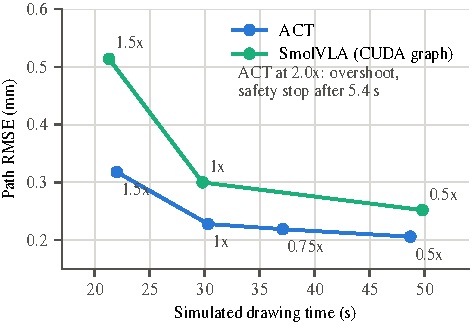
\includegraphics[width=\columnwidth]{figures/speed.pdf}
  \caption{Speed against accuracy on the gold cat (interactive runner): the step scale $\alpha$ of
  Eq.~(\ref{eq:step}) relative to the default 0.5 is shown next to each point. ACT keeps most of its accuracy up
  to 1.0; SmolVLA degrades sooner.}
  \label{fig:speed}
\end{figure}

\textbf{Speed.} Scaling ACT's applied step (Fig.~\ref{fig:speed}) from 0.5 to 0.75 of the prediction keeps RMSE within 6\% (0.206 to
0.219\mm) and cuts simulated time by 24\%; 1.0 gives +11\% error for 38\% less time; 2.0 overshoots and trips
the 5\mm safety stop, consistent with the curvature-speed trade-off reported for
Piktor-O-Bot~\cite{csempesz2024piktor}. SmolVLA has no faster setting within 10\%.

\textbf{Physical arm.} The twin-trained ACT policy ran on the lab arm without fine-tuning. In a 30-drawing batch
(five per class, not the gold-set drawings) every drawing finished, at 0.532\mm mean path RMSE
(0.421 to 0.622\mm), 2.7$\times$ the twin (Table~\ref{tab:realclass}, Fig.~\ref{fig:twinreal}). Stalls were the main failure mode: 14 of
30 drawings needed at least one nudge to resume (26 in total), always mid-stroke where waypoints are dense; the pen
sat about 0.5\mm beside the path and corrected only sideways. Three face portraits drawn with markers
(Table~\ref{tab:real}) finished at 0.497\mm measured RMSE, using an automatic 0.5\,s stall release instead of
nudges.

\textbf{Scoring the ink.} The arm's reported tip says where the arm believes the pen is, not what reached the
paper. We therefore score the sheet itself: the page is found in an overhead photograph and rectified to
millimetres, the ink is thinned to a centre line, and the ink is fitted to the plan by a trimmed rigid
transform (ink onto plan, so missing ink cannot drag the fit). On portrait A the ink lies 0.43 to 0.48\mm from
the plan on average, in line with the reported tip error, and 90\% of the plan has ink within 2\mm.
Portrait B scores lower for a reason the arm's log cannot see: the long hair below the shoulders inked faintly,
so only 71\% of the plan is covered. The photograph's 0.6\mm pixels bound this measurement; flatbed scans are
planned for the paired real-arm study.

\begin{figure}[t]
  \centering
  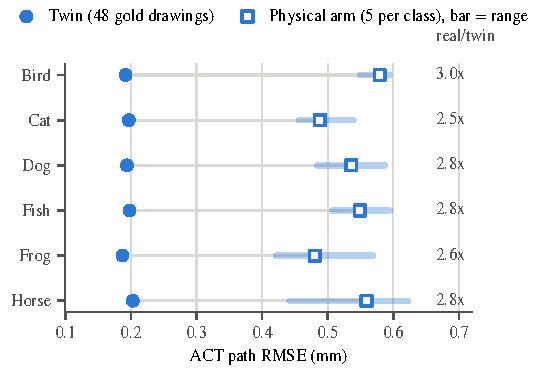
\includegraphics[width=\columnwidth]{figures/twin_vs_real.pdf}
  \caption{ACT path RMSE per class in the twin (gold set) and on the physical arm (five drawings per class,
  range shown). The real arm is 2.5 to 3.0$\times$ the twin in every class. Drawings differ between the two sets,
  so the comparison is per class, not paired.}
  \label{fig:twinreal}
\end{figure}

\begin{table}[t]
\centering
\caption{ACT on the physical arm, 30 animal drawings (five per class). Path RMSE in mm.}
\label{tab:realclass}
\setlength{\tabcolsep}{3pt}
\begin{tabular}{lcccc}
\toprule
Class & RMSE mean (range) & Worst point & Time (s) & Nudges / drawing \\
\midrule
Bird  & 0.579 (0.549-0.594) & 1.54 & 76  & 0.8 \\
Cat   & 0.488 (0.456-0.539) & 1.53 & 96  & 1.6 \\
Dog   & 0.536 (0.484-0.587) & 1.47 & 72  & 0.0 \\
Fish  & 0.549 (0.507-0.595) & 1.49 & 102 & 0.4 \\
Frog  & 0.480 (0.421-0.569) & 1.51 & 100 & 0.4 \\
Horse & 0.559 (0.442-0.622) & 1.54 & 117 & 2.0 \\
\midrule
All   & 0.532 (0.421-0.622) & 1.54 & 94  & 0.87 \\
\bottomrule
\end{tabular}
\end{table}

\begin{table}[t]
\centering
\caption{Face portraits on the physical arm with ACT and a marker. RMSE, p95 and max are measured from the
arm's reported tip at 10\,Hz; chamfer and coverage are measured from the ink in an overhead photograph. mm.}
\label{tab:real}
\setlength{\tabcolsep}{2.2pt}
\begin{tabular}{lcccccc}
\toprule
Run & RMSE & p95 & Max & Chamfer & Cov.\,2\,mm & min \\
\midrule
A (48 strokes), used sheet  & 0.486 & 0.912 & 1.306 & 0.74 & 90\% & 8.5 \\
A (48 strokes), clean sheet & 0.514 & 0.966 & 1.305 & 0.67 & 90\% & 8.3 \\
B (59 strokes), clean sheet & 0.490 & 0.905 & 1.273 & 2.13 & 71\% & 9.7 \\
\bottomrule
\end{tabular}
\end{table}

%======================================================================
\section{Discussion and Limitations}
%======================================================================

\textbf{Why ACT beats its own teacher.} ACT is trained on IK labels yet outperforms IK because the labels are
kinematic: they describe where the arm should go, not IK's gravity-induced sag, and the noise-injected episodes
teach correction. Training on physics rollouts of IK imported IK's error. Querying a short path window at
60\,Hz also replaces IK's stop-and-settle with continuous motion, which is where the jerk and the tremor come
from. The streaming IK result shows that continuous motion alone is not enough: an IK solver chasing a moving
target cuts corners and stays jerky, while the policy has learned from noise-injected labels how to correct
toward the path.

\textbf{Sim-to-real gap.} The 2.7$\times$ gap is consistent across classes, which points to a systematic
cause rather than content. Candidates we observed are a non-level sheet (line weight varies across the page),
pen compliance, the arm's own position controller differing from the twin's servo, and dense-waypoint stalls.
Fitting the paper plane from a three-point touch and training on stalled states are the next steps.

\textbf{What the pipeline does not preserve.} FLUX passes the referee reliably but redraws the subject in a
generic pose: in our generator study its median silhouette IoU with the source photo was about 0.2, against
0.78 to 0.91 for OmniGen2's non-blank drawings, and facing direction matched in 65\% of cases. The drawings are
recognisably the right animal, not a tracing of the photo. Lower diffusion strength or contour conditioning is
the obvious next step.

\textbf{Baseline strength.} We compare against the waypoint-gated IK controller the system shipped with and
a streaming IK that shares ACT's progress rule; an optimisation-based tracker (for example model-predictive
contouring control) and the vendor's own Cartesian motion commands on the real arm are stronger baselines we have
not yet run.

\textbf{Limitations.} Each controller was run once per drawing; ACT was trained with three seeds; the other policies with one. The real-arm batch used different drawings
from the gold set and relied on nudges, so it is not a controlled paired comparison. The path metric is
geometric; ink scoring from photographs covers only three portraits so far, and perceived quality (a user study)
is future work. The IK baseline is
tolerance-gated and its timeouts could be reduced by tuning. Real-arm portraits take 8 to 10\,min, against
43\,s to 2\,min for systems built for exhibition speed~\cite{wang2019robocodraw,gao2020aisketcher,nasrat2023artistic};
our runs used the default step scale and stall releases, not a speed-tuned setting. The hybrid supervisor and
the camera policies were evaluated on 12 drawings in the interactive runner only.

\textbf{Reproducibility.} Every number in this paper comes from per-run metric files kept with the code: the
configuration hash, checkpoint and runner of each run are recorded, and one script regenerates all figures and
the statistics in Tables~\ref{tab:gold} and~\ref{tab:class}.

%======================================================================
\section{Conclusion}
%======================================================================

WildTrace turns photographs into robot pen drawings end to end. A compact ACT path follower trained only on
kinematic IK labels draws held-out content more accurately, more reliably and more smoothly than the IK
solver that labelled it, is robust to paper placement, and transfers to a physical xArm 7 at about half a
millimetre RMSE. A streaming IK with the same progress rule gains almost nothing, so the accuracy comes from
learning. A fine-tuned VLA re-planned every tick is slightly more accurate again but jerkier and slower to query,
and a simple supervisor makes either policy robust to missed ink. Closing the remaining sim-to-real gap is our next goal.

\bibliographystyle{IEEEtran}
\bibliography{refs}

\end{document}
